\documentclass[aspectratio=169, 11pt]{beamer}

% ── Theme: Clean white background ──
\usetheme{default}
\usecolortheme{default}
\setbeamercolor{structure}{fg=black!80}
\setbeamercolor{frametitle}{fg=black!90, bg=white}
\setbeamercolor{title}{fg=black!90}
\setbeamercolor{subtitle}{fg=black!60}
\setbeamercolor{author}{fg=black!70}
\setbeamercolor{date}{fg=black!50}
\setbeamercolor{normal text}{fg=black!85, bg=white}
\setbeamercolor{block title}{fg=white, bg=black!70}
\setbeamercolor{block body}{fg=black!85, bg=black!5}
\setbeamercolor{block title alerted}{fg=white, bg=red!65!black}
\setbeamercolor{block body alerted}{fg=black!85, bg=red!5}
\setbeamercolor{block title example}{fg=white, bg=green!45!black}
\setbeamercolor{block body example}{fg=black!85, bg=green!5}
\setbeamercolor{itemize item}{fg=black!70}
\setbeamercolor{itemize subitem}{fg=black!60}
\setbeamercolor{enumerate item}{fg=black!70}
\setbeamertemplate{navigation symbols}{}
\setbeamertemplate{footline}{%
  \hfill\insertframenumber/\inserttotalframenumber\hspace*{6pt}\vspace{4pt}%
}
\setbeamertemplate{date}{}
\setbeamerfont{frametitle}{size=\large, series=\bfseries}

% ── Packages ──
\usepackage[utf8]{inputenc}
\usepackage[T1]{fontenc}
\usepackage{amsmath,amssymb}
\usepackage{graphicx}
\usepackage{tikz}
\usetikzlibrary{shapes.geometric, arrows.meta, positioning, fit, backgrounds, calc}
\usepackage{booktabs}
\usepackage{multirow}
\usepackage{tabularx}
\usepackage{hyperref}
\usepackage{xcolor}
\usepackage{array}

% ── TikZ styles (matching report) ──
\tikzset{
  block/.style={rectangle, draw, rounded corners, minimum height=0.7cm,
    minimum width=1.8cm, align=center, font=\scriptsize, fill=blue!8},
  decision/.style={diamond, draw, aspect=2.2, align=center,
    font=\scriptsize, fill=yellow!10, inner sep=1pt},
  action/.style={rectangle, draw, rounded corners, minimum height=0.6cm,
    minimum width=1.5cm, align=center, font=\scriptsize, fill=green!10},
  alert/.style={rectangle, draw, rounded corners, minimum height=0.6cm,
    minimum width=1.5cm, align=center, font=\scriptsize, fill=red!10},
  phase/.style={rectangle, draw, rounded corners, minimum height=0.8cm,
    minimum width=2.2cm, align=center, font=\small\bfseries, fill=blue!15},
  arr/.style={-{Stealth[length=2mm]}, thick},
  biarr/.style={{Stealth[length=2mm]}-{Stealth[length=2mm]}, thick},
}

% ── Title info ──
\title{Extending Kubernetes Self-Healing\\for Networking Failures}
\subtitle{CS331 - Computer Networks Project}
\author{
  Arpan Gupta (24110051) \\ 
  Buha Deep Maheshbhai (24110082) \\ 
  Param Tanna (24110236) \\  
  Ramji Purwar (24110287) \\ 
  Rathod Yuvraj Rajubhai (24110293) \\ 
  Solanki Viraj Rajeshbhai (24110348) \\
}
\date[]{}

\begin{document}

% SLIDE 1 — Title
\begin{frame}[plain]
  \titlepage
\end{frame}

% SLIDE 2 — Problem Statement & Objective
\begin{frame}{Problem Statement \& Objective}

\textbf{Problem:} Kubernetes heals container crashes but is \alert{blind to network-layer failures}.

\begin{itemize}
  \item CNI plugin crashes $\to$ pods stuck in \texttt{ContainerCreating}
  \item CoreDNS degradation $\to$ silent DNS resolution failures
  \item Overlay tunnel drops $\to$ cross-node traffic silently fails
  \item Pods show \texttt{Running (1/1 Ready)} while network is dead
\end{itemize}

\vspace{6pt}

\begin{block}{Objective}
Build a \textbf{custom Kubernetes operator} that continuously monitors and auto-remediates three critical network subsystems:
\begin{enumerate}
  \item \textbf{CNI plugin health} (Calico IPAM exhaustion \& agent failures)
  \item \textbf{CoreDNS availability} (scale-to-zero, corrupted upstreams, latency spikes)
  \item \textbf{Pod-to-pod connectivity} (overlay tunnel drops \& cross-node routing)
\end{enumerate}
\end{block}

\end{frame}

% SLIDE 3 — Limitation of Kubernetes
\begin{frame}{Limitation of Kubernetes}

\begin{columns}[T]
\begin{column}{0.31\textwidth}
\begin{block}{CNI Plugin (Calico)}
\footnotesize
\begin{itemize}
  \item \texttt{calico-node} agent crash
  \item IPAM pool exhaustion
  \item Disabled IPPool
\end{itemize}
\end{block}
\end{column}

\begin{column}{0.31\textwidth}
\begin{block}{CoreDNS}
\footnotesize
\begin{itemize}
  \item Replicas scaled to zero
  \item CPU throttling ($\leq$5\,m)
  \item Latency spikes (${>}$1000\,ms)
  \item Corrupted upstream forward
\end{itemize}
\end{block}
\end{column}

\begin{column}{0.31\textwidth}
\begin{block}{Pod-to-Pod}
\footnotesize
\begin{itemize}
  \item Virtual interface (\texttt{veth}) down
  \item Overlay tunnel (IPIP) drop
\end{itemize}
\end{block}
\end{column}
\end{columns}

\end{frame}

% SLIDE 4 — System Architecture Overview
\begin{frame}{System Architecture}

\begin{columns}[T]
\begin{column}{0.52\textwidth}
\centering
\resizebox{0.95\textwidth}{!}{%
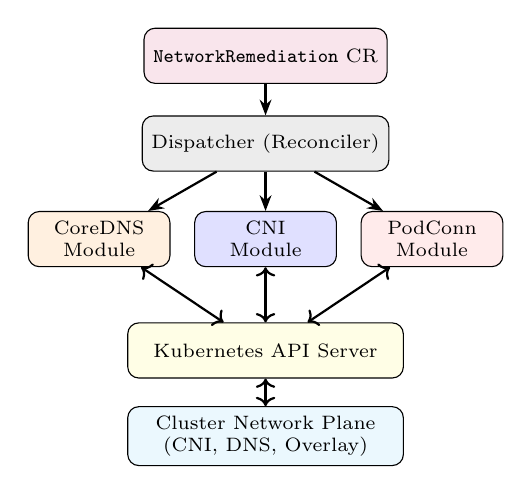
\begin{tikzpicture}[node distance=0.3cm and 0.2cm]
  % CR
  \node[block, fill=purple!10, minimum width=2.8cm] (cr) {\texttt{NetworkRemediation} CR};
  
  % Dispatcher
  \node[block, fill=gray!15, minimum width=2.8cm, below=0.4cm of cr] (disp) {Dispatcher (Reconciler)};
  
  % Modules
  \node[block, fill=blue!12, below=0.5cm of disp] (cni) {CNI\\Module};
  \node[block, fill=orange!12, left=0.3cm of cni] (dns) {CoreDNS\\Module};
  \node[block, fill=red!8, right=0.3cm of cni] (pc) {PodConn\\Module};
  
  % Kubernetes API
  \node[block, fill=yellow!10, minimum width=3.5cm, below=0.7cm of cni] (api) {Kubernetes API Server};
  
  % Network plane
  \node[block, fill=cyan!8, minimum width=3.5cm, below=0.35cm of api] (net) {Cluster Network Plane\\(CNI, DNS, Overlay)};
  
  \draw[arr] (cr) -- (disp);
  \draw[arr] (disp) -- (dns);
  \draw[arr] (disp) -- (cni);
  \draw[arr] (disp) -- (pc);
  \draw[arr, <->] (dns) -- (api);
  \draw[arr, <->] (cni) -- (api);
  \draw[arr, <->] (pc) -- (api);
  \draw[arr, <->] (api) -- (net);
\end{tikzpicture}%
}
\end{column}
\end{columns}

\end{frame}

% SLIDE 6 — Pipeline: Check → Evaluate → Remediate
\begin{frame}{Three-Phase Pipeline: Check $\to$ Evaluate $\to$ Remediate}

\begin{columns}[T]
\begin{column}{0.48\textwidth}
\centering
\resizebox{0.85\textwidth}{!}{%
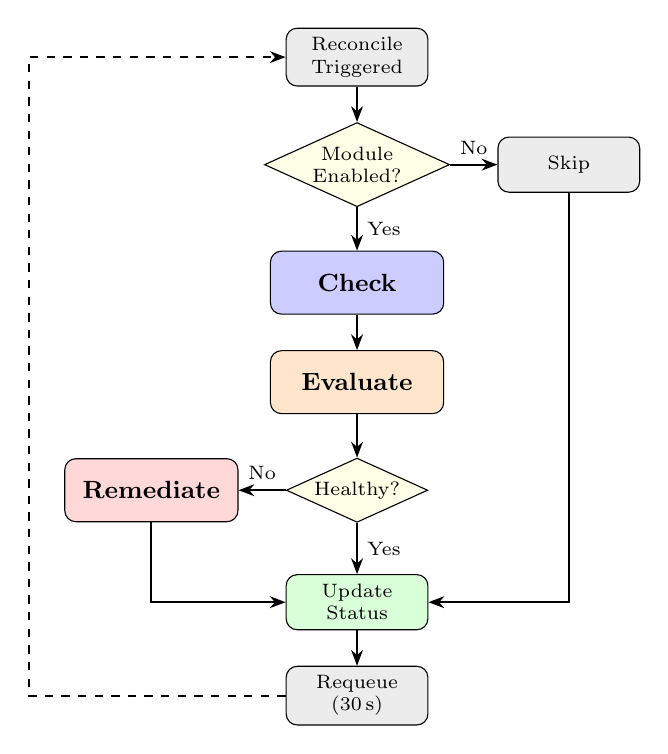
\begin{tikzpicture}[node distance=0.45cm and 0.5cm]
  \node[block, fill=gray!15] (trigger) {Reconcile\\Triggered};
  \node[decision, below=0.45cm of trigger] (enabled) {Module\\Enabled?};
  \node[block, fill=gray!15, right=0.6cm of enabled] (skip) {Skip};
  \node[phase, fill=blue!20, below=0.55cm of enabled] (check) {Check};
  \node[phase, fill=orange!20, below=0.45cm of check] (eval) {Evaluate};
  \node[decision, below=0.55cm of eval] (healthy) {Healthy?};
  \node[phase, fill=red!15, left=0.6cm of healthy] (rem) {Remediate};
  \node[block, fill=green!15, below=0.65cm of healthy] (status) {Update\\Status};
  \node[block, fill=gray!15, below=0.45cm of status] (requeue) {Requeue\\(30\,s)};

  \coordinate (loopleft) at ($(rem.west)+(-0.45cm, 0)$);

  \draw[arr] (trigger) -- (enabled);
  \draw[arr] (enabled) -- node[above, font=\scriptsize] {No} (skip);
  \draw[arr] (enabled) -- node[right, font=\scriptsize] {Yes} (check);
  \draw[arr] (check) -- (eval);
  \draw[arr] (eval) -- (healthy);
  \draw[arr] (healthy) -- node[right, font=\scriptsize] {Yes} (status);
  \draw[arr] (healthy) -- node[above, font=\scriptsize] {No} (rem);
  \draw[arr] (rem.south) |- (status.west);
  \draw[arr] (skip.south) |- (status.east);
  \draw[arr] (status) -- (requeue);
  \draw[arr, dashed] (requeue.west) -- (requeue.west -| loopleft) -- (trigger.west -| loopleft) -- (trigger.west);
\end{tikzpicture}%
}
\end{column}

\begin{column}{0.50\textwidth}
\vspace{6pt}
\begin{block}{Check - Signal Gathering}
\footnotesize
Collects raw network telemetry: pod statuses, DaemonSet health, IPAM allocations, DNS latency, active probe results. \emph{No decisions made.}
\end{block}

\begin{block}{Evaluate - Failure Classification}
\footnotesize
Analyzes signals against configurable thresholds. Classifies severity: \texttt{info}, \texttt{warning}, \texttt{critical}. Prevents false positives.
\end{block}

\begin{block}{Remediate - Corrective Action}
\footnotesize
Executes minimum K8s API mutations: pod deletions, deployment scaling, ConfigMap patches, node taints, workload evictions.
\end{block}
\end{column}
\end{columns}

\end{frame}

% SLIDE 7 — CRD Configuration
\begin{frame}{CRD-Driven Configuration}

\begin{columns}[T]
\begin{column}{0.54\textwidth}
\centering
\resizebox{\columnwidth}{!}{%
\renewcommand{\arraystretch}{1.15}
\setlength{\tabcolsep}{3pt}
\scriptsize
\begin{tabular}{@{}l l l@{}}
\toprule
\textbf{Module} & \textbf{Key Parameter} & \textbf{Default} \\
\midrule
\multirow{3}{*}{CNI} & \texttt{stuckPodThresholdSec} & 60\,s \\
                     & \texttt{ipamUsageThreshold\%} & 80\% \\
                     & \texttt{calicoNodeLabel} & \texttt{calico-node} \\
\midrule
\multirow{4}{*}{CoreDNS} & \texttt{expectedReplicas} & 2 \\
                         & \texttt{latencyThresholdMs} & 150\,ms \\
                         & \texttt{autoHealReplicas} & true \\
                         & \texttt{autoHealConfigMap} & true \\
\midrule
\multirow{3}{*}{\shortstack[l]{Pod\\Conn}} & \texttt{consecutiveFailThreshold} & 3 \\
                                           & \texttt{autoRemediationEnabled} & true \\
                                           & \texttt{maxRestartAttempts} & 2 \\
\bottomrule
\end{tabular}%
}
\end{column}

\begin{column}{0.43\textwidth}
\footnotesize
\textbf{Key Design Points:}
\begin{itemize}
  \item Single \textbf{cluster-scoped} CRD: \texttt{NetworkRemediation} (\texttt{v1alpha1})
  \item Each module independently \textbf{toggleable} via \texttt{enabled} field
  \item Safety guardrails: cooldown windows, escalation limits, failure thresholds
  \item Supports \textbf{audit-only mode}: observe and log without mutating
\end{itemize}
\end{column}
\end{columns}

\end{frame}

% SLIDE 8 — CNI Module
\begin{frame}{CNI Module: Detection \& Remediation}

\begin{columns}[T]
\begin{column}{0.48\textwidth}
\footnotesize
\textbf{Detection Signals:}
\begin{enumerate}
  \item \textbf{DaemonSet health:} \texttt{desiredNumberScheduled} vs \texttt{numberReady}
  \item \textbf{Stuck workload pods:} \texttt{Pending} phase + empty \texttt{podIP} exceeding threshold
  \item \textbf{CNI event correlation:} \texttt{FailedCreatePodSandBox} warning events with CNI/IPAM signatures
  \item \textbf{IPAM capacity:} Calico \texttt{IPPool} and \texttt{IPAMBlock} CRDs for disabled pools and exhausted blocks
\end{enumerate}
\end{column}

\begin{column}{0.48\textwidth}
\footnotesize
\textbf{Evaluation Priority Order:}
\begin{enumerate}
  \item Unready calico-node $\to$ \texttt{critical}, restart agents
  \item Disabled IPPool + stuck pods $\to$ \texttt{critical}, re-enable pool
  \item Stuck pods + CNI errors $\to$ \texttt{critical}, evict pods
  \item IPAM usage $\geq$ threshold $\to$ \texttt{warning}, log only
\end{enumerate}

\vspace{4pt}
\textbf{Remediation Actions:}
\begin{itemize}
  \item[\textcolor{green!60!black}{$\blacksquare$}] \textbf{Restart:} Delete unready \texttt{calico-node} pods
  \item[\textcolor{yellow!70!black}{$\blacksquare$}] \textbf{Re-enable:} Patch \texttt{spec.disabled} $\to$ \texttt{false}
  \item[\textcolor{red!60!black}{$\blacksquare$}] \textbf{Evict:} Delete stranded pods for rescheduling
\end{itemize}
\end{column}
\end{columns}

\end{frame}

% SLIDE 9 — CoreDNS Module
\begin{frame}{CoreDNS Module: Detection \& Remediation}

\begin{columns}[T]
\begin{column}{0.48\textwidth}
\footnotesize
\textbf{Detection Signals:}
\begin{enumerate}
  \item \textbf{Replica availability:} \texttt{availableReplicas} vs \texttt{expectedReplicas}
  \item \textbf{Pod readiness:} \texttt{CrashLoopBackOff}, \texttt{Error}, or unready states
  \item \textbf{DNS query latency:} via Prometheus metrics
  \[
    \text{Latency} = \frac{\texttt{rate(sum[1m])}}{\texttt{rate(count[1m])}}
  \]
  \item \textbf{Upstream validation:} Corefile \texttt{forward} targets checked against RFC~5737 bad subnets
  \item \textbf{Resource starvation:} CPU limits $\leq$5\,m causing latency spikes
\end{enumerate}
\end{column}

\begin{column}{0.48\textwidth}
\footnotesize
\textbf{Remediation Actions:}
\begin{itemize}
  \item \textbf{Scale recovery:} Patch replicas back to \texttt{expectedReplicas}
  \item \textbf{Pod restart:} Delete unready/crashlooping pods
  \item \textbf{ConfigMap repair:} Replace corrupted \texttt{forward} targets with fallbacks (\texttt{/etc/resolv.conf}, \texttt{8.8.8.8})
  \item \textbf{Resource restoration:} Reset CPU limits to 100\,m baseline
\end{itemize}

\vspace{4pt}
\textbf{Safety Mechanisms:}
\begin{itemize}
  \item Independent toggles: \texttt{autoHealReplicas}, \texttt{autoHealConfigMap}
  \item 30\,s cooldown window per remediation type
\end{itemize}
\end{column}
\end{columns}

\end{frame}

% SLIDE 10 — Pod Connectivity: Pingmesh Ring
\begin{frame}{Pod Connectivity Module: $O(N)$ Pingmesh Ring Probing}

\begin{columns}[T]
\begin{column}{0.50\textwidth}
\centering
\resizebox{0.9\textwidth}{!}{%
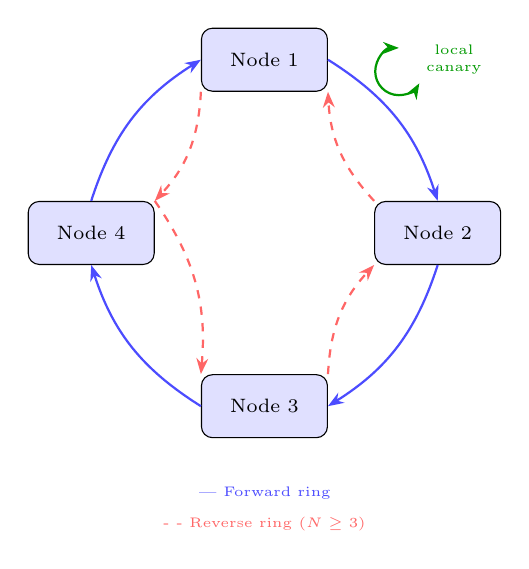
\begin{tikzpicture}
  % Ring of 4 nodes
  \def\radius{2.2cm}
  \node[block, fill=blue!12, minimum width=1.6cm, minimum height=0.8cm] (n1) at (90:\radius) {Node 1};
  \node[block, fill=blue!12, minimum width=1.6cm, minimum height=0.8cm] (n2) at (0:\radius) {Node 2};
  \node[block, fill=blue!12, minimum width=1.6cm, minimum height=0.8cm] (n3) at (270:\radius) {Node 3};
  \node[block, fill=blue!12, minimum width=1.6cm, minimum height=0.8cm] (n4) at (180:\radius) {Node 4};

  % Forward ring (outer, blue)
  \draw[arr, blue!70, thick] (n1.east) to[bend left=20] node[font=\tiny, right, blue!70] {} (n2.north);
  \draw[arr, blue!70, thick] (n2.south) to[bend left=20] (n3.east);
  \draw[arr, blue!70, thick] (n3.west) to[bend left=20] (n4.south);
  \draw[arr, blue!70, thick] (n4.north) to[bend left=20] (n1.west);

  % Reverse ring (inner, red dashed)
  \draw[arr, red!60, thick, dashed] (n2.north west) to[bend left=20] (n1.south east);
  \draw[arr, red!60, thick, dashed] (n3.north east) to[bend left=20] (n2.south west);
  \draw[arr, red!60, thick, dashed] (n4.north east) to[bend left=20] (n3.north west);
  \draw[arr, red!60, thick, dashed] (n1.south west) to[bend left=20] (n4.north east);

  % Legend
  \node[font=\tiny, blue!70] at (0, -3.3) {--- Forward ring};
  \node[font=\tiny, red!60] at (0, -3.7) {- - Reverse ring $(N \geq 3)$};

  % Intra-node canary
  \draw[biarr, green!60!black] ([xshift=0.9cm, yshift=0.15cm]n1.east) arc (90:330:0.3cm);
  \node[font=\tiny, green!60!black, align=center] at ([xshift=1.6cm, yshift=0.0cm]n1.east) {local\\canary};
\end{tikzpicture}%
}
\end{column}

\begin{column}{0.47\textwidth}
\footnotesize
\textbf{Topology Design:}
\begin{itemize}
  \item Nodes sorted lexicographically, connected in a ring
  \item Forward: $Node_i \to Node_{(i+1) \bmod N}$
  \item Reverse: $Node_i \to Node_{(i-1+N) \bmod N}$
\end{itemize}

\vspace{4pt}
\textbf{Scalability:}
\begin{itemize}
  \item Exactly $2N$ inter-node probes $\to$ $O(N)$
  \item vs.\ full-mesh probing: $O(N^2)$
  \item $+$ $O(1)$ intra-node canary per node (veth, bridge, iptables FORWARD chain)
\end{itemize}

\vspace{4pt}
\textbf{Adapted from:}\\
Microsoft Pingmesh [SIGCOMM 2015]
\end{column}
\end{columns}

\end{frame}

% SLIDE 11 — Three-Tier Triangulation
\begin{frame}{Three-Tier Triangulation for Root-Cause Isolation}

\begin{columns}[T]
\begin{column}{0.50\textwidth}
\centering
\resizebox{\textwidth}{!}{%
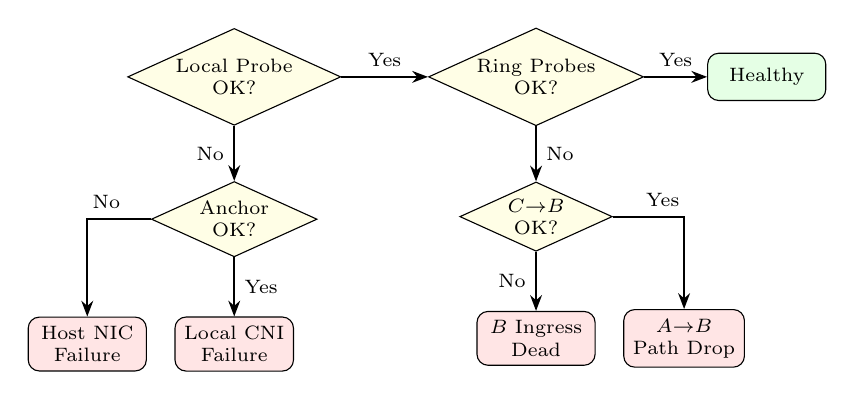
\begin{tikzpicture}[every node/.style={font=\scriptsize}]
  % Top row
  \node[decision] (local) {Local Probe\\OK?};
  \node[decision, right=1.1cm of local] (ring) {Ring Probes\\OK?};
  \node[action, right=0.8cm of ring] (ok) {Healthy};

  % Middle row
  \node[decision, below=0.7cm of local] (anchor1) {Anchor\\OK?};
  \node[decision, below=0.7cm of ring] (tri) {$C{\to}B$\\OK?};

  % Bottom row
  \node[alert, below=0.75cm of anchor1] (localcni) {Local CNI\\Failure};
  \node[alert, left=0.35cm of localcni] (blackhole) {Host NIC\\Failure};

  \node[alert, below=0.75cm of tri] (ingress) {$B$ Ingress\\Dead};
  \node[alert, right=0.35cm of ingress] (path) {$A{\to}B$\\Path Drop};

  % Connections
  \draw[arr] (local) -- node[above, font=\scriptsize] {Yes} (ring);
  \draw[arr] (local) -- node[left, font=\scriptsize] {No} (anchor1);
  \draw[arr] (ring) -- node[above, font=\scriptsize] {Yes} (ok);
  \draw[arr] (ring) -- node[right, font=\scriptsize] {No} (tri);

  \draw[arr] (anchor1) -- node[right, font=\scriptsize] {Yes} (localcni);
  \draw[arr] (anchor1.west) -| node[above, font=\scriptsize, pos=0.35] {No} (blackhole.north);

  \draw[arr] (tri) -- node[left, font=\scriptsize] {No} (ingress);
  \draw[arr] (tri.east) -| node[above, font=\scriptsize, pos=0.35] {Yes} (path.north);
\end{tikzpicture}%
}
\end{column}

\begin{column}{0.47\textwidth}
\footnotesize
\textbf{Tier 1 - Local CNI Validation:}\\
Local probe fails but anchors (gateway, CoreDNS) reachable $\to$ local CNI issue

\vspace{3pt}
\textbf{Tier 2 - Inter-Node Triangulation:}\\
$A \not\to B$: check if $C \to B$. All peers fail $\to$ $B$ ingress dead. Only $A$ fails $\to$ asymmetric path drop

\vspace{3pt}
\textbf{Tier 3 - Anchor Corroboration:}\\
For small clusters ($N < 3$): probes against gateway, \texttt{kube-apiserver} disambiguate host vs tunnel failures

\vspace{4pt}
\textbf{Hierarchical Remediation:}
\begin{enumerate}
  \item CNI Agent Restart (max 2 attempts)
  \item Node Taint \& Cordon (\texttt{NoSchedule})
  \item Workload Drain (Eviction API)
\end{enumerate}
\end{column}
\end{columns}

\end{frame}

% SLIDE 12 — Experimental Setup
\begin{frame}{Experimental Setup}

\begin{columns}[T]
\begin{column}{0.45\textwidth}
\footnotesize
\textbf{Cluster Environment:}
\vspace{4pt}
\renewcommand{\arraystretch}{1.15}
\setlength{\tabcolsep}{4pt}
\begin{tabular}{@{}l l@{}}
\toprule
\textbf{Component} & \textbf{Configuration} \\
\midrule
Cluster & Minikube (Docker), 2 nodes \\
Resources/Node & 2 vCPUs, 4096\,MB RAM \\
CNI Plugin & Calico (DaemonSet) \\
DNS Server & CoreDNS (2 replicas) \\
K8s Version & v1.31+ \\
Operator & Kubebuilder v4.15+, Go 1.24+ \\
\bottomrule
\end{tabular}
\end{column}

\begin{column}{0.52\textwidth}
\footnotesize
\textbf{Fault-Injection Methodology:}
\begin{enumerate}
  \item Establish \textbf{healthy cluster baseline}
  \item \textbf{Inject} specific network fault; observe native K8s behavior (no operator)
  \item \textbf{Enable operator}; verify automated detection and recovery
\end{enumerate}

\vspace{4pt}
\textbf{Test Workloads:}
\begin{itemize}
  \item \texttt{backend-api} - HTTP service (2 replicas, spread across nodes)
  \item \texttt{frontend-probe} - continuous HTTP poller
  \item \texttt{dns-checker} - DNS resolution verifier
\end{itemize}
\end{column}
\end{columns}

\end{frame}

% % SLIDE 14 — Non-Functional Testing Parameters
% \begin{frame}{Non-Functional Testing Parameters}

% \begin{columns}[T]
% \begin{column}{0.48\textwidth}
% \textbf{Detection \& Recovery Performance:}
% \begin{itemize}
%   \item \textbf{Detection latency:} $<$30\,s (single reconcile cycle)
%   \item \textbf{Remediation time:} 30--60\,s across all modules
%   \item \textbf{Probe scalability:} $O(N)$ via Pingmesh ring topology
%   \item \textbf{False positive rate:} 0\% (three-tier triangulation prevents misdiagnosis)
% \end{itemize}

% \vspace{6pt}
% \textbf{Reliability:}
% \begin{itemize}
%   \item \textbf{Reconcile interval:} 30\,s (configurable)
%   \item \textbf{Cooldown windows:} 30\,s per remediation type to prevent restart thrashing
%   \item \textbf{Consecutive failure threshold:} 3 (avoids reacting to transient issues)
% \end{itemize}
% \end{column}

% \begin{column}{0.48\textwidth}
% \textbf{Safety \& Configurability:}
% \begin{itemize}
%   \item \textbf{Audit-only mode:} disable auto-heal per module, observe and log only
%   \item \textbf{Escalation limits:} \texttt{maxRestartAttempts} (default: 2) before escalation to taint/drain
%   \item \textbf{Independent toggles:} each remediation type gated separately
%   \item \textbf{PDB compliance:} workload drain respects PodDisruptionBudgets
% \end{itemize}

% \vspace{6pt}
% \textbf{Resource Efficiency:}
% \begin{itemize}
%   \item Single operator pod manages all three modules
%   \item No additional DaemonSet or sidecar required
%   \item Minimal API server load (periodic polling, not watch-heavy)
% \end{itemize}
% \end{column}
% \end{columns}

% \end{frame}

% SLIDE 15 — Challenges Faced
% \begin{frame}{Challenges Faced}

% \begin{columns}[T]
% \begin{column}{0.48\textwidth}

% \begin{block}{1. Multi-Node Minikube Setup}
% Minikube defaults to single-node; required \texttt{-{}-nodes=2} with Calico CNI for cross-node testing. Default CNI (kindnet) doesn't support IPIP tunnels or IPPool CRDs.
% \end{block}

% \begin{block}{2. Calico Bootstrap Timing}
% CNI agent needs time to establish BGP mesh on startup. Operator must tolerate transient \texttt{NotReady} states during cluster bootstrap without triggering false remediation.
% \end{block}

% \begin{block}{3. IPAM CRD Access Permissions}
% Calico IPPool/IPAMBlock are third-party CRDs not auto-discovered by controller-runtime. Required custom RBAC rules and explicit scheme registration.
% \end{block}

% \end{column}

% \begin{column}{0.48\textwidth}

% \begin{block}{4. Prometheus Dependency for DNS Latency}
% CoreDNS latency monitoring requires Prometheus deployment and scraping. Implemented fallback to direct DNS probing when Prometheus is unavailable.
% \end{block}

% \begin{block}{5. Tunnel Interface Restoration}
% Simply running \texttt{ip link set tunl0 up} is insufficient --- CNI agent restart required to rebuild routing tables and rebind tunnel interfaces.
% \end{block}

% \begin{block}{6. Reconcile Loop Race Conditions}
% Multiple modules modifying cluster state simultaneously can conflict. Resolved with per-module cooldown windows and sequential pipeline execution.
% \end{block}

% \end{column}
% \end{columns}

% \end{frame}

% SLIDE 16 — Conclusion & Future Work
\begin{frame}{Conclusion \& Future Work}

\begin{columns}[T]
\begin{column}{0.48\textwidth}
\footnotesize
\textbf{Conclusion:}
\begin{itemize}
  \item Extends K8s self-healing to the \textbf{network data plane}
  \item Modular \textbf{Check $\to$ Evaluate $\to$ Remediate} pipeline
  \item \textbf{$O(N)$ Pingmesh ring probing} + 3-tier triangulation
  \item Validated across \textbf{8/8 fault experiments} (30--60\,s recovery)
\end{itemize}
\end{column}

\begin{column}{0.48\textwidth}
\footnotesize
\textbf{Future Work:}
\begin{itemize}
  \item \textbf{Alertmanager:} Slack, PagerDuty notifications
  \item \textbf{eBPF Probing:} Kernel-level introspection with lower overhead
  \item \textbf{ML Anomaly Detection:} Time-series DNS \& latency models
  \item \textbf{Multi-Cluster:} Cross-cluster network mesh healing
\end{itemize}
\end{column}
\end{columns}

\end{frame}

% SLIDE 17 — References
% \begin{frame}[allowframebreaks]{References}
% \footnotesize
% \begin{thebibliography}{10}

% \bibitem{pingmesh2015}
% C.~Guo et~al.,
% \newblock ``Pingmesh: A Large-Scale System for Data Center Network Latency Measurement and Analysis,''
% \newblock in \emph{Proc.\ ACM SIGCOMM}, pp.~139--152, 2015.

% \bibitem{netbouncer2019}
% C.~Tan et~al.,
% \newblock ``NetBouncer: Active Device and Link Failure Localization in Data Center Networks,''
% \newblock in \emph{Proc.\ USENIX NSDI}, pp.~599--614, 2019.

% \bibitem{k8s-docs}
% The Kubernetes Authors,
% \newblock ``Kubernetes Documentation,''
% \newblock \url{https://kubernetes.io/docs/}, 2024.

% \bibitem{calico-docs}
% Tigera, Inc.,
% \newblock ``Calico Open Source Networking and Network Security,''
% \newblock \url{https://docs.tigera.io/calico/latest/about/}, 2024.

% \bibitem{coredns-docs}
% CoreDNS Authors,
% \newblock ``CoreDNS: DNS and Service Discovery,''
% \newblock \url{https://coredns.io/manual/toc/}, 2024.

% \bibitem{kubebuilder}
% The Kubernetes Authors,
% \newblock ``The Kubebuilder Book,''
% \newblock \url{https://book.kubebuilder.io/}, 2024.

% \bibitem{goldpinger}
% Bloomberg,
% \newblock ``Goldpinger: Debugging Tool for Kubernetes Cluster Networking,''
% \newblock \url{https://github.com/bloomberg/goldpinger}, 2023.

% \bibitem{cni-spec}
% CNI Authors,
% \newblock ``Container Network Interface (CNI) Specification,''
% \newblock \url{https://www.cni.dev/docs/spec/}, 2024.

% \bibitem{rfc5737}
% J.~Arkko, M.~Cotton, L.~Vegoda,
% \newblock ``IPv4 Address Blocks Reserved for Documentation,''
% \newblock RFC~5737, IETF, 2010.

% \end{thebibliography}
% \end{frame}

% SLIDE 18 — Thank You
{
\setbeamercolor{background canvas}{bg=white}
\begin{frame}[plain,c]
\centering

{\Huge\bfseries Thank You!}

\vspace{16pt}

\vspace{24pt}
{\small
\begin{tabular}{ccc}

  Arpan Gupta (24110051) \\ 
  Buha Deep Maheshbhai (24110082) \\ 
  Param Tanna (24110236) \\  
  Ramji Purwar (24110287) \\ 
  Rathod Yuvraj Rajubhai (24110293) \\ 
  Solanki Viraj Rajeshbhai (24110348) \\
\end{tabular}
}

\end{frame}
}

\end{document}
